\documentclass[aspectratio=169,12pt]{beamer}
\usepackage[utf8]{inputenc}
\usepackage{amsmath, amssymb}
\usepackage{booktabs}
\usepackage{colortbl}
\usepackage{hyperref}
\usepackage{makecell}
\usepackage{ragged2e}
\usepackage{tikz}
\usetikzlibrary{arrows.meta, positioning, shapes.geometric, calc, tikzmark, shapes.misc, fit, decorations.pathreplacing, matrix}
\usepackage{tcolorbox}
\usepackage{array}
\usepackage{listings}
\usepackage{pgfkeys}
\usepackage{adjustbox}
\usepackage[normalem]{ulem}
\usetheme{Madrid}
\usecolortheme{default}

% Custom colors
\definecolor{mygreen}{RGB}{0,150,0}
\definecolor{myblue}{RGB}{0,100,200}
\definecolor{myred}{RGB}{200,0,0}
\definecolor{mygray}{RGB}{100,100,100}

% Additional colors for bit field diagrams
\definecolor{fieldpurple}{RGB}{200,180,255}
\definecolor{fieldblue}{RGB}{180,220,255}
\definecolor{fieldgreen}{RGB}{180,255,180}
\definecolor{fieldyellow}{RGB}{255,255,180}
\definecolor{fieldorange}{RGB}{255,220,180}
\definecolor{fieldpink}{RGB}{255,200,230}
\definecolor{fieldgray}{RGB}{220,220,220}
\definecolor{fieldcyan}{RGB}{180,255,255}
\definecolor{fieldred}{RGB}{255,180,180}

% Macro for creating bit field diagrams  
\newcommand{\drawbitfield}[2]{
  % #1: total bits (e.g., 64)
  % #2: comma-separated list of field specifications
  \begin{tikzpicture}[
    scale=0.8,
    cell/.style={rectangle, draw=black, thick, minimum height=0.8cm, font=\tiny},
    label/.style={font=\scriptsize},
    arrow/.style={->, >=stealth, thick}
  ]
    % Total width calculation
    \pgfmathsetmacro{\bitwidth}{0.25}
    \pgfmathsetmacro{\totalwidth}{#1*\bitwidth}
    
    % Draw main border first
    \draw[very thick] (0, 0) rectangle (\totalwidth, 0.8);
    
    % Process each field
    \foreach \spec in {#2} {
      % Parse the specification
      \pgfkeys{/bitfield/.cd, default, \spec}
      \pgfmathtruncatemacro{\startbit}{\fieldstartbit}
      \pgfmathtruncatemacro{\endbit}{\fieldendbit}
      
      % Calculate positions
      \pgfmathsetmacro{\startx}{\startbit*\bitwidth}
      \pgfmathsetmacro{\endx}{(\endbit+1)*\bitwidth}
      \pgfmathsetmacro{\fieldwidth}{\endx-\startx}
      \pgfmathsetmacro{\centerx}{(\startx+\endx)/2}
      
      % Draw field box with color
      \fill[\fieldcolor!30] (\startx, 0) rectangle (\endx, 0.8);
      \draw[thick] (\startx, 0) -- (\startx, 0.8);
      \ifnum\endbit<#1
        \ifnum\endbit<63
          \draw[thick] (\endx, 0) -- (\endx, 0.8);
        \fi
      \fi
      
      % Add field text
      \node[font=\tiny] at (\centerx, 0.4) {\fieldshortname};
      
      % Add bit numbers below
      \ifnum\startbit=\endbit
        \node[below, label] at (\centerx, 0) {\startbit};
      \else
        \node[below, label] at (\startx, 0) {\startbit};
        \node[below, label] at (\endx, 0) {\endbit};
      \fi
      
      % Add long description with arrow if not empty
      \def\emptystring{}
      \ifx\fieldlongname\emptystring\else
        % Calculate label position (stagger heights)
        \pgfmathsetmacro{\labely}{1.2 + 0.4*mod(\startbit/5, 4)}
        \node[above, align=center, label, text=\fieldcolor!70!black] 
              (label-\startbit) at (\centerx, \labely) {\fieldlongname};
        \draw[arrow, \fieldcolor!60!black] (label-\startbit.south) -- (\centerx, 0.8);
      \fi
    }
    
    % Add overall bit range labels
    \node[below, label] at (0, -0.5) {0};
    \pgfmathtruncatemacro{\maxbit}{#1-1}
    \node[below, label] at (\totalwidth, -0.5) {\maxbit};
  \end{tikzpicture}
}

% pgfkeys for field specifications
\pgfkeys{
  /bitfield/.is family, /bitfield,
  default/.style = {
    startbit = 0,
    endbit = 0,
    shortname = {},
    longname = {},
    color = fieldgray
  },
  startbit/.estore in = \fieldstartbit,
  endbit/.estore in = \fieldendbit,
  shortname/.estore in = \fieldshortname,
  longname/.estore in = \fieldlongname,
  color/.estore in = \fieldcolor
}

% Unified macro for virtual address breakdown with up to 6 fields
% Usage: \vmaddressbreakdown{signbits}{pml4bits}{pdpbits}{dirbits}{tablebits}{offsetbits}
% Pass 0 for fields that should be skipped
% When DIR=0 and TABLE=0, the last field becomes OFFSET
% When DIR>0 and TABLE=0, the last field becomes DIR/OFFSET combined
% When both DIR>0 and TABLE>0, they are separate fields with OFFSET last
\newcommand{\vmaddressbreakdown}[6]{%
    \begin{tikzpicture}[
        section/.style={draw, very thick, minimum height=0.7cm},
        bitnumber/.style={font=\tiny},
        sectionlabel/.style={font=\scriptsize},
        baseline=(current bounding box.center)
    ]
    \pgfmathsetmacro{\bitwidth}{0.17}
    \pgfmathsetmacro{\xpos}{0}
    \pgfmathtruncatemacro{\currentbit}{63}

    % Field 1: Sign extension
    \ifnum#1>0
        \pgfmathtruncatemacro{\fldstart}{\currentbit}
        \pgfmathtruncatemacro{\fldend}{\currentbit - #1 + 1}
        \pgfmathsetmacro{\fldwidth}{#1 * \bitwidth}

        \node[section, fill=gray!40, minimum width=\fldwidth cm] (f) at (\xpos + \fldwidth/2, 0) {};
        \node[sectionlabel, align=center] at (f.center) {Sign\\Ext};
        \node[bitnumber] at ($(f.south west) + (2mm,-1mm)$) {\fldstart};
        \node[bitnumber] at ($(f.south east) + (-2mm,-1mm)$) {\fldend};

        \pgfmathsetmacro{\xpos}{\xpos + \fldwidth}
        \pgfmathtruncatemacro{\currentbit}{\fldend - 1}
    \fi

    % Field 2: PML4
    \ifnum#2>0
        \pgfmathtruncatemacro{\fldstart}{\currentbit}
        \pgfmathtruncatemacro{\fldend}{\currentbit - #2 + 1}
        \pgfmathsetmacro{\fldwidth}{#2 * \bitwidth}

        \node[section, fill=orange!40, minimum width=\fldwidth cm] (f) at (\xpos + \fldwidth/2, 0) {};
        \node[sectionlabel, align=center] at (f.center) {PML4};
        \node[bitnumber] at ($(f.south west) + (2mm,-1mm)$) {\fldstart};
        \node[bitnumber] at ($(f.south east) + (-2mm,-1mm)$) {\fldend};

        \pgfmathsetmacro{\xpos}{\xpos + \fldwidth}
        \pgfmathtruncatemacro{\currentbit}{\fldend - 1}
    \fi

    % Field 3: PDP
    \ifnum#3>0
        \pgfmathtruncatemacro{\fldstart}{\currentbit}
        \pgfmathtruncatemacro{\fldend}{\currentbit - #3 + 1}
        \pgfmathsetmacro{\fldwidth}{#3 * \bitwidth}

        \node[section, fill=blue!40, minimum width=\fldwidth cm] (f) at (\xpos + \fldwidth/2, 0) {};
        \node[sectionlabel, align=center] at (f.center) {PDP};
        \node[bitnumber] at ($(f.south west) + (2mm,-1mm)$) {\fldstart};
        \node[bitnumber] at ($(f.south east) + (-2mm,-1mm)$) {\fldend};

        \pgfmathsetmacro{\xpos}{\xpos + \fldwidth}
        \pgfmathtruncatemacro{\currentbit}{\fldend - 1}
    \fi

    % Field 4: DIR
    \ifnum#4>0
        \pgfmathtruncatemacro{\fldstart}{\currentbit}
        \pgfmathtruncatemacro{\fldend}{\currentbit - #4 + 1}
        \pgfmathsetmacro{\fldwidth}{#4 * \bitwidth}

        \node[section, fill=green!40, minimum width=\fldwidth cm] (f) at (\xpos + \fldwidth/2, 0) {};
        \node[sectionlabel, align=center] at (f.center) {DIR};
        \node[bitnumber] at ($(f.south west) + (2mm,-1mm)$) {\fldstart};
        \node[bitnumber] at ($(f.south east) + (-2mm,-1mm)$) {\fldend};

        \pgfmathsetmacro{\xpos}{\xpos + \fldwidth}
        \pgfmathtruncatemacro{\currentbit}{\fldend - 1}
    \fi

    % Field 5: TABLE
    \ifnum#5>0
        \pgfmathtruncatemacro{\fldstart}{\currentbit}
        \pgfmathtruncatemacro{\fldend}{\currentbit - #5 + 1}
        \pgfmathsetmacro{\fldwidth}{#5 * \bitwidth}

        \node[section, fill=yellow!40, minimum width=\fldwidth cm] (f) at (\xpos + \fldwidth/2, 0) {};
        \node[sectionlabel, align=center] at (f.center) {TABLE};
        \node[bitnumber] at ($(f.south west) + (2mm,-1mm)$) {\fldstart};
        \node[bitnumber] at ($(f.south east) + (-2mm,-1mm)$) {\fldend};

        \pgfmathsetmacro{\xpos}{\xpos + \fldwidth}
        \pgfmathtruncatemacro{\currentbit}{\fldend - 1}
    \fi

    % Field 6: OFFSET (always present)
    \ifnum#6>0
        \pgfmathtruncatemacro{\fldstart}{\currentbit}
        \pgfmathtruncatemacro{\fldend}{\currentbit - #6 + 1}
        \pgfmathsetmacro{\fldwidth}{#6 * \bitwidth}

        \node[section, fill=red!40, minimum width=\fldwidth cm] (f) at (\xpos + \fldwidth/2, 0) {};
        \node[sectionlabel, align=center] at (f.center) {OFFSET};
        \node[bitnumber] at ($(f.south west) + (2mm,-1mm)$) {\fldstart};
        \node[bitnumber] at ($(f.south east) + (-2mm,-1mm)$) {\fldend};
    \fi

    \end{tikzpicture}
}

\title{x86 Virtual Memory and TLB}
\author{Computer Architecture 234267}
\date{2025, Recitation \#11}



\begin{document}

\begin{frame}
\titlepage
\end{frame}

% Slide 2: X86 Paging Introduction
\begin{frame}{X86 Paging}
\begin{itemize}
    \item For 32-bit addressing with 4KB page size, a full page table would require 4MB
    \item Most processes use only a small amount of memory
    \item The overhead of 4MB per process is expensive and unnecessary
    \item In X86, there are multiple levels of translation tables organized in a tree structure
    \item We allocate translation tables dynamically, only when actually needed
\end{itemize}
\end{frame}

% Slide 3: 32-bit Mode Page Mapping
\begin{frame}{32-bit Mode: 4KB / 4MB Page Mapping}
\begin{itemize}
    \item 2-level hierarchical mapping: Page Directories and Page Tables
    \item 4KB aligned pages
    \item PDE (Page Directory Entry) contains:
    \begin{itemize}
        \item Present bit (0 = page fault)
        \item Page size (4KB or 4MB)
        \item CR4.PSE=1 $\Rightarrow$ both 4MB \& 4KB pages supported
        \item Separate TLBs for different page sizes
    \end{itemize}
\end{itemize}

\vspace{1em}
Linear Address Space breakdown:
\begin{itemize}
    \item 4KB Page: DIR[31:22] | TABLE[21:12] | OFFSET[11:0]
    \item 4MB Page: DIR[31:22] | OFFSET[21:0]
\end{itemize}
\end{frame}

% Slide 4: PDE and PTE Format
\begin{frame}{32-bit Mode: PDE and PTE Format}
\centering
\textbf{Page Directory Entry (4KB page table)}\\[0.5em]
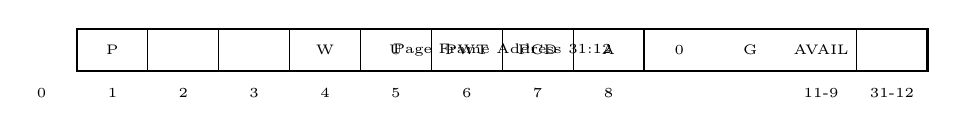
\begin{tikzpicture}[scale=0.9]
    % PDE structure
    \draw[thick] (0,0) rectangle (12,0.6);
    \foreach \x/\txt in {0/0,1/1,2/2,3/3,4/4,5/5,6/6,7/7,8/8,11/{11-9},12/{31-12}} {
        \draw (\x,0) -- (\x,0.6);
        \node[below] at (\x-0.5,-0.1) {\tiny \txt};
    }
    \node at (6,0.3) {\tiny Page Frame Address 31:12};
    \node at (10.5,0.3) {\tiny AVAIL};
    \node at (9.5,0.3) {\tiny G};
    \node at (8.5,0.3) {\tiny 0};
    \node at (7.5,0.3) {\tiny A};
    \node at (6.5,0.3) {\tiny PCD};
    \node at (5.5,0.3) {\tiny PWT};
    \node at (4.5,0.3) {\tiny U};
    \node at (3.5,0.3) {\tiny W};
    \node at (0.5,0.3) {\tiny P};
\end{tikzpicture}

\vspace{1em}
\textbf{Page Table Entry}\\[0.5em]
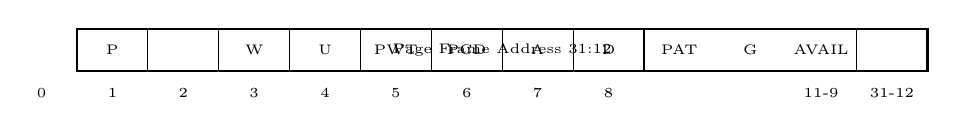
\begin{tikzpicture}[scale=0.9]
    % PTE structure
    \draw[thick] (0,0) rectangle (12,0.6);
    \foreach \x/\txt in {0/0,1/1,2/2,3/3,4/4,5/5,6/6,7/7,8/8,11/{11-9},12/{31-12}} {
        \draw (\x,0) -- (\x,0.6);
        \node[below] at (\x-0.5,-0.1) {\tiny \txt};
    }
    \node at (6,0.3) {\tiny Page Frame Address 31:12};
    \node at (10.5,0.3) {\tiny AVAIL};
    \node at (9.5,0.3) {\tiny G};
    \node at (8.5,0.3) {\tiny PAT};
    \node at (7.5,0.3) {\tiny D};
    \node at (6.5,0.3) {\tiny A};
    \node at (5.5,0.3) {\tiny PCD};
    \node at (4.5,0.3) {\tiny PWT};
    \node at (3.5,0.3) {\tiny U};
    \node at (2.5,0.3) {\tiny W};
    \node at (0.5,0.3) {\tiny P};
\end{tikzpicture}

\vspace{1em}
\small
Key: P=Present, W=Writable, U=User/Supervisor, PWT=Write-Through,\\
PCD=Cache Disable, A=Accessed, D=Dirty, G=Global, PAT=Page Attribute Table
\end{frame}

% Slide 5: Intel 64-bit PTE Format  
\begin{frame}{Intel 64-bit Page Table Entry (PTE)}
\centering
\textbf{64-bit Mode PTE Format}\\[0.5em]

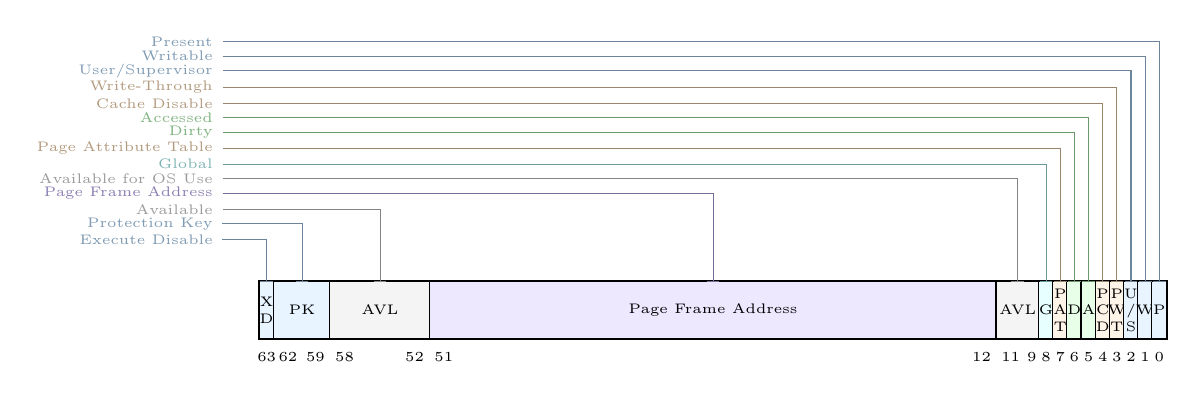
\begin{tikzpicture}[scale=0.18, font=\tiny]
  % Define constants
  \def\boxheight{4}
  \def\bitwidth{1}
  
  % Define colors by functionality
  % Protection-related: blue
  % Caching-related: orange  
  % Access tracking: green
  % Software available: gray
  % Address: purple
  
  % Define key coordinates as base references
  \coordinate (origin) at (0,0);
  \coordinate (topright) at (64,\boxheight);
  
  % Draw outer border
  \draw[very thick] (origin) rectangle (topright);
  
  % Define field boundaries using coordinates
  % Working from MSB (63) to LSB (0), left to right
  \coordinate (b63) at (0,0);               % MSB position
  \coordinate (b62) at ($(b63) + (1,0)$);   % XD is 1 bit wide
  \coordinate (b59) at ($(b62) + (4,0)$);   % PK is 4 bits wide (62-59)
  \coordinate (b52) at ($(b59) + (7,0)$);   % Available is 7 bits wide (58-52)
  \coordinate (b12) at ($(b52) + (40,0)$);  % PFA is 40 bits wide (51-12)
  \coordinate (b9) at ($(b12) + (3,0)$);    % AVL is 3 bits wide (11-9)
  \coordinate (b8) at ($(b9) + (1,0)$);     % G is 1 bit wide (bit 8)
  \coordinate (b7) at ($(b8) + (1,0)$);     % PAT is 1 bit wide (bit 7)
  \coordinate (b6) at ($(b7) + (1,0)$);     % D is 1 bit wide (bit 6)
  \coordinate (b5) at ($(b6) + (1,0)$);     % A is 1 bit wide (bit 5)
  \coordinate (b4) at ($(b5) + (1,0)$);     % PCD is 1 bit wide (bit 4)
  \coordinate (b3) at ($(b4) + (1,0)$);     % PWT is 1 bit wide (bit 3)
  \coordinate (b2) at ($(b3) + (1,0)$);     % U/S is 1 bit wide (bit 2)
  \coordinate (b1) at ($(b2) + (1,0)$);     % W is 1 bit wide (bit 1)
  \coordinate (b0) at ($(b1) + (1,0)$);     % P is 1 bit wide (bit 0)
  
  % XD bit (63) - using coordinates
  \fill[fieldblue!30] (b63) rectangle ($(b62) + (0,\boxheight)$);
  \draw[thick] (b62) -- ($(b62) + (0,\boxheight)$);
  \node[align=center] at ($(b63)!0.5!(b62) + (0,\boxheight/2)$) {X\\D};
  \node[below] at ($(b63)!0.5!(b62) + (0,-0.3)$) {63};
  
  % Protection Key (59-62) - relative to previous
  \fill[fieldblue!30] (b62) rectangle ($(b59) + (0,\boxheight)$);
  \draw[thick] (b59) -- ($(b59) + (0,\boxheight)$);
  \node at ($(b62)!0.5!(b59) + (0,\boxheight/2)$) {PK};
  \node[below] at ($(b62) + (1,-0.3)$) {62};
  
  % Available bits (52-58) - relative positioning
  \fill[fieldgray!30] (b59) rectangle ($(b52) + (0,\boxheight)$);
  \draw[thick] (b52) -- ($(b52) + (0,\boxheight)$);
  \node[align=center] at ($(b59)!0.5!(b52) + (0,\boxheight/2)$) {AVL};
  \node[below] (b58lbl) at ($(b59) + (1,-0.3)$) {58};
  \node[left=0cm of b58lbl, anchor=east, inner sep=0pt] {59};
  
  % Page Frame Address (12-51) - relative positioning
  \fill[fieldpurple!30] (b52) rectangle ($(b12) + (0,\boxheight)$);
  \draw[thick] (b12) -- ($(b12) + (0,\boxheight)$);
  \node at ($(b52)!0.5!(b12) + (0,\boxheight/2)$) {Page Frame Address};
  \node[below] (b51lbl) at ($(b52) + (1,-0.3)$) {51};
  \node[left=0cm of b51lbl, anchor=east, inner sep=0pt] {52};
  
  % AVL bits (9-11) - relative
  \fill[fieldgray!30] (b12) rectangle ($(b9) + (0,\boxheight)$);
  \draw[thick] (b9) -- ($(b9) + (0,\boxheight)$);
  \node at ($(b12)!0.5!(b9) + (0,\boxheight/2)$) {AVL};
  \node[below] (b11lbl) at ($(b12) + (1,-0.3)$) {11};
  \node[left=0cm of b11lbl, anchor=east, inner sep=0pt] {12};
  
  % G bit (8) - relative
  \fill[fieldcyan!30] (b9) rectangle ($(b8) + (0,\boxheight)$);
  \draw[thick] (b8) -- ($(b8) + (0,\boxheight)$);
  \node at ($(b9)!0.5!(b8) + (0,\boxheight/2)$) {G};
  \node[below] (b8lbl) at ($(b9)!0.5!(b8) + (0,-0.3)$) {8};
  \node[left=-2pt of b8lbl, anchor=east, inner sep=0pt] {9};
  
  % PAT bit (7) - relative
  \fill[fieldorange!30] (b8) rectangle ($(b7) + (0,\boxheight)$);
  \draw[thick] (b7) -- ($(b7) + (0,\boxheight)$);
  \node[align=center] at ($(b8)!0.5!(b7) + (0,\boxheight/2)$) {P\\A\\T};
  \node[below] at ($(b8)!0.5!(b7) + (0,-0.3)$) {7};
  
  % D bit (6) - relative
  \fill[fieldgreen!30] (b7) rectangle ($(b6) + (0,\boxheight)$);
  \draw[thick] (b6) -- ($(b6) + (0,\boxheight)$);
  \node at ($(b7)!0.5!(b6) + (0,\boxheight/2)$) {D};
  \node[below] at ($(b7)!0.5!(b6) + (0,-0.3)$) {6};
  
  % A bit (5) - relative
  \fill[fieldgreen!30] (b6) rectangle ($(b5) + (0,\boxheight)$);
  \draw[thick] (b5) -- ($(b5) + (0,\boxheight)$);
  \node at ($(b6)!0.5!(b5) + (0,\boxheight/2)$) {A};
  \node[below] at ($(b6)!0.5!(b5) + (0,-0.3)$) {5};
  
  % PCD bit (4) - relative
  \fill[fieldorange!30] (b5) rectangle ($(b4) + (0,\boxheight)$);
  \draw[thick] (b4) -- ($(b4) + (0,\boxheight)$);
  \node[align=center] at ($(b5)!0.5!(b4) + (0,\boxheight/2)$) {P\\C\\D};
  \node[below] at ($(b5)!0.5!(b4) + (0,-0.3)$) {4};
  
  % PWT bit (3) - relative
  \fill[fieldorange!30] (b4) rectangle ($(b3) + (0,\boxheight)$);
  \draw[thick] (b3) -- ($(b3) + (0,\boxheight)$);
  \node[align=center] at ($(b4)!0.5!(b3) + (0,\boxheight/2)$) {P\\W\\T};
  \node[below] at ($(b4)!0.5!(b3) + (0,-0.3)$) {3};
  
  % U/S bit (2) - relative
  \fill[fieldblue!30] (b3) rectangle ($(b2) + (0,\boxheight)$);
  \draw[thick] (b2) -- ($(b2) + (0,\boxheight)$);
  \node[align=center] at ($(b3)!0.5!(b2) + (0,\boxheight/2)$) {U\\/\\S};
  \node[below] at ($(b3)!0.5!(b2) + (0,-0.3)$) {2};
  
  % W bit (1) - relative
  \fill[fieldblue!30] (b2) rectangle ($(b1) + (0,\boxheight)$);
  \draw[thick] (b1) -- ($(b1) + (0,\boxheight)$);
  \node at ($(b2)!0.5!(b1) + (0,\boxheight/2)$) {W};
  \node[below] at ($(b2)!0.5!(b1) + (0,-0.3)$) {1};
  
  % P bit (0) - LSB on the right
  \fill[fieldblue!30] (b1) rectangle ($(b0) + (0,\boxheight)$);
  \node at ($(b1)!0.5!(b0) + (0,\boxheight/2)$) {P};
  \node[below] at ($(b1)!0.5!(b0) + (0,-0.3)$) {0};
  
  % Add descriptive labels below with -| arrows - using relative positioning
  % Base y-coordinate for labels
  \coordinate (labelbase) at ($(origin) + (0,-2)$);

  % Labels ordered from MSB (63) to LSB (0), stacked vertically
  % Start with XD bit (63) at the top
  \node[below, align=left, text=fieldblue!70!black] (lblXD) at ($(b63) + (-8,8)$) {Execute Disable};
  \draw[-|, fieldblue!60!black] (lblXD.east) -| ($(b63.north)!0.5!(b62.north) + (0,\boxheight)$);

  % Protection Key (59-62)
  \node[below, align=left, text=fieldblue!70!black, above=0mm of lblXD.east, anchor=south east] (lblPK) {Protection Key};
  \draw[-|, fieldblue!60!black] (lblPK.east) -| ($(b62.north)!0.5!(b59.north) + (0, \boxheight)$);
  
  % Available (52-58)
  \node[below, align=left, text=fieldgray!70!black, above=0mm of lblPK.east, anchor=south east] (lblAVL2) {Available};
  \draw[-|, fieldgray!60!black] (lblAVL2.east) -| ($(b59.north)!0.5!(b52.north) + (0, \boxheight)$);
  
  % Physical Page Frame Address (12-51)
  \node[below, align=left, text=fieldpurple!70!black, above=0mm of lblAVL2.east, anchor=south east] (lblPFA) {Page Frame Address};
  \draw[-|, fieldpurple!60!black] (lblPFA.east) -| ($(b52.north)!0.5!(b12.north) + (0, \boxheight)$);
  
  % Available for OS Use (9-11)
  \node[below, align=left, text=fieldgray!70!black, above=0mm of lblPFA.east, anchor=south east] (lblAVL1) {Available for OS Use};
  \draw[-|, fieldgray!60!black] (lblAVL1.east) -| ($(b12.north)!0.5!(b9.north) + (0, \boxheight)$);
  
  % Global bit (8)
  \node[below, align=left, text=fieldcyan!70!black, above=0mm of lblAVL1.east, anchor=south east] (lblG) {Global};
  \draw[-|, fieldcyan!60!black] (lblG.east) -| ($(b9.north)!0.5!(b8.north) + (0, \boxheight)$);
  
  % Page Attribute Table (7)
  \node[below, align=left, text=fieldorange!70!black, above=0mm of lblG.east, anchor=south east] (lblPAT) {Page Attribute Table};
  \draw[-|, fieldorange!60!black] (lblPAT.east) -| ($(b8.north)!0.5!(b7.north) + (0, \boxheight)$);
  
  % Dirty bit (6)
  \node[below, align=left, text=fieldgreen!70!black, above=0mm of lblPAT.east, anchor=south east] (lblD) {Dirty};
  \draw[-|, fieldgreen!60!black] (lblD.east) -| ($(b7.north)!0.5!(b6.north) + (0, \boxheight)$);
  
  % Accessed bit (5)
  \node[below, align=left, text=fieldgreen!70!black, above=0mm of lblD.east, anchor=south east] (lblA) {Accessed};
  \draw[-|, fieldgreen!60!black] (lblA.east) -| ($(b6.north)!0.5!(b5.north) + (0, \boxheight)$);
  
  % Cache Disable (4)
  \node[below, align=left, text=fieldorange!70!black, above=0mm of lblA.east, anchor=south east] (lblPCD) {Cache Disable};
  \draw[-|, fieldorange!60!black] (lblPCD.east) -| ($(b5.north)!0.5!(b4.north) + (0, \boxheight)$);
  
  % Write-Through (3)
  \node[below, align=left, text=fieldorange!70!black, above=0mm of lblPCD.east, anchor=south east] (lblPWT) {Write-Through};
  \draw[-|, fieldorange!60!black] (lblPWT.east) -| ($(b4.north)!0.5!(b3.north) + (0, \boxheight)$);
  
  % User/Supervisor (2)
  \node[below, align=left, text=fieldblue!70!black, above=0mm of lblPWT.east, anchor=south east] (lblUS) {User/Supervisor};
  \draw[-|, fieldblue!60!black] (lblUS.east) -| ($(b3.north)!0.5!(b2.north) + (0, \boxheight)$);
  
  % Writable (1)
  \node[below, align=left, text=fieldblue!70!black, above=0mm of lblUS.east, anchor=south east] (lblW) {Writable};
  \draw[-|, fieldblue!60!black] (lblW.east) -| ($(b2.north)!0.5!(b1.north) + (0, \boxheight)$);
  
  % Present (0)
  \node[below, align=left, text=fieldblue!70!black, above=0mm of lblW.east, anchor=south east] (lblP) {Present};
  \draw[-|, fieldblue!60!black] (lblP.east) -| ($(b1.north)!0.5!(b0.north) + (0, \boxheight)$);
\end{tikzpicture}

\vspace{1em}
\small
\begin{itemize}
  \item 64-bit entries support 52-bit physical addresses
  \item Protection keys (PK) provide additional access control
  \item XD bit prevents code execution from data pages
\end{itemize}
\end{frame}

% Slide 6: 64-bit Mode Page Mapping
\begin{frame}{4KB Page Mapping in 64-bit Mode}
\begin{itemize}
    \item Introduced in 2003 with AMD Opteron
    \item 4-level hierarchy: PML4, PDP, DIR, TABLE
    \item 512 entries per table (9 bits addressing)
    \item 48 bits of virtual address space (256 TB)
    \item 40 bits of physical address space (1 TB)
\end{itemize}

\vspace{1em}
\textbf{Linear Address breakdown (4KB page):} \vmaddressbreakdown{16}{9}{9}{9}{9}{12}
\end{frame}

% Slide 6: Large Pages in 64-bit Mode
\begin{frame}{Large Pages in 64-bit Mode}
\textbf{2MB Page Mapping:}
\begin{itemize}
    \item Linear Address: \vmaddressbreakdown{16}{9}{9}{9}{0}{21}
    \item Page size: $2^{21}$ = 2MB
\end{itemize}

\vspace{1em}
\textbf{1GB Page Mapping:}
\begin{itemize}
    \item Linear Address: \vmaddressbreakdown{16}{9}{9}{0}{0}{30}
    \item Page size: $2^{30}$ = 1GB
\end{itemize}
\end{frame}

% Slide 7: Question 1 Setup
\begin{frame}{Question 1}
Core similar to X86 in 64-bit mode:
\begin{itemize}
    \item Support Small Pages (PTE) and Large Pages (DIR)
    \item Page table size = small page size
    \item Entry size in all hierarchies = 16 bytes
\end{itemize}

\vspace{0.5em}
\textbf{Address format:}
\begin{center}
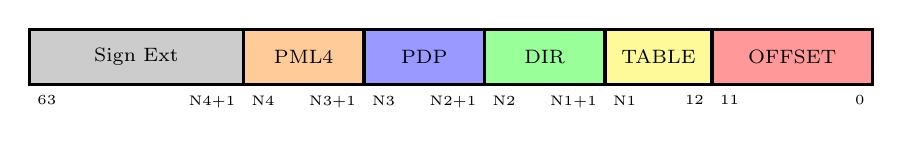
\begin{tikzpicture}[
    section/.style={draw, very thick, minimum height=0.7cm},
    bitnumber/.style={font=\tiny, anchor=south},
    sectionlabel/.style={font=\scriptsize}
]
\pgfmathsetmacro{\bitwidth}{0.17}
\pgfmathsetmacro{\xpos}{0}

% Field widths (using standard x86 9-bit fields)
\def\signbits{16}
\def\pmlfourbits{9}
\def\pdpbits{9}
\def\dirbits{9}
\def\tablebits{8}
\def\offsetbits{12}

% Sign Extension
\pgfmathsetmacro{\fldwidth}{\signbits * \bitwidth}
\node[section, fill=gray!40, minimum width=\fldwidth cm] (f1) at (\xpos + \fldwidth/2, 0) {};
\node[sectionlabel, align=center] at (f1.center) {Sign Ext};
\node[bitnumber, anchor=north west] at (f1.south west) {63};
\node[bitnumber, anchor=north east] at (f1.south east) {N4+1};
\pgfmathsetmacro{\xpos}{\xpos + \fldwidth}

% PML4
\pgfmathsetmacro{\fldwidth}{\pmlfourbits * \bitwidth}
\node[section, fill=orange!40, minimum width=\fldwidth cm] (f2) at (\xpos + \fldwidth/2, 0) {};
\node[sectionlabel, align=center] at (f2.center) {PML4};
\node[bitnumber, anchor=north west] at (f2.south west) {N4};
\node[bitnumber, anchor=north east] at (f2.south east) {N3+1};
\pgfmathsetmacro{\xpos}{\xpos + \fldwidth}

% PDP
\pgfmathsetmacro{\fldwidth}{\pdpbits * \bitwidth}
\node[section, fill=blue!40, minimum width=\fldwidth cm] (f3) at (\xpos + \fldwidth/2, 0) {};
\node[sectionlabel, align=center] at (f3.center) {PDP};
\node[bitnumber, anchor=north west] at (f3.south west) {N3};
\node[bitnumber, anchor=north east] at (f3.south east) {N2+1};
\pgfmathsetmacro{\xpos}{\xpos + \fldwidth}

% DIR
\pgfmathsetmacro{\fldwidth}{\dirbits * \bitwidth}
\node[section, fill=green!40, minimum width=\fldwidth cm] (f4) at (\xpos + \fldwidth/2, 0) {};
\node[sectionlabel, align=center] at (f4.center) {DIR};
\node[bitnumber, anchor=north west] at (f4.south west) {N2};
\node[bitnumber, anchor=north east] at (f4.south east) {N1+1};
\pgfmathsetmacro{\xpos}{\xpos + \fldwidth}

% TABLE
\pgfmathsetmacro{\fldwidth}{\tablebits * \bitwidth}
\node[section, fill=yellow!40, minimum width=\fldwidth cm] (f5) at (\xpos + \fldwidth/2, 0) {};
\node[sectionlabel, align=center] at (f5.center) {TABLE};
\node[bitnumber, anchor=north west] at (f5.south west) {N1};
\node[bitnumber, anchor=north east] at (f5.south east) {12};
\pgfmathsetmacro{\xpos}{\xpos + \fldwidth}

% OFFSET
\pgfmathsetmacro{\fldwidth}{\offsetbits * \bitwidth}
\node[section, fill=red!40, minimum width=\fldwidth cm] (f6) at (\xpos + \fldwidth/2, 0) {};
\node[sectionlabel, align=center] at (f6.center) {OFFSET};
\node[bitnumber, anchor=north west] at (f6.south west) {11};
\node[bitnumber, anchor=north east] at (f6.south east) {0};
\end{tikzpicture}
\end{center}

\vspace{0.5em}
\textbf{Questions:}
\begin{enumerate}
    \item What is the size of a small page?
    \item How many entries are in each Page Table?
    \item What are the values of N1, N2, N3, and N4?
    \item What is the size of a large page?
\end{enumerate}
\end{frame}

% Slide 8: Question 1 Solution
\begin{frame}{Question 1: Solution (a)}
\begin{enumerate}
    \item \textbf{Small page size}
    \begin{itemize}
        \item[] 12 bits in offset field $\Rightarrow 2^{12}$ = 4KB
    \end{itemize}
    \item \textbf{Entries per Page Table}
    \begin{itemize}
        \item Page Table size = Page Size = 4KB
        \item PTE = 16B
        \item Entries = $\frac{\text{4KB}}{\text{16B}} = \frac{2^{12}}{2^4} = 2^8$ = 256 entries
    \end{itemize}
\end{enumerate}
\end{frame}

\begin{frame}{Question 1: Solution (b)}
\begin{enumerate}
    \setcounter{enumi}{2}
    \item \textbf{Values of N1, N2, N3, N4}
    \begin{itemize}
        \item 256 entries $\Rightarrow$ 8 bits to address them
    \end{itemize}
    \begin{center}
        \begin{tabular}{lcl}
            TABLE [19:12] & $\Rightarrow$ & N1 = 19\\
            DIR [27:20]   & $\Rightarrow$ & N2 = 27\\
            PDP [35:28]   & $\Rightarrow$ & N3 = 35\\
            PML4 [43:36]  & $\Rightarrow$ & N4 = 43
        \end{tabular}
    \end{center}

    \item \textbf{Large page size}
    \begin{itemize}
        \item Large pages pointed by DIR, offset is [19:0]
        \item Size = $2^{20}$ = 1MB
    \end{itemize}
\end{enumerate}
\end{frame}

% Slide 9: TLB Introduction
\begin{frame}{Translation Lookaside Buffer (TLB)}
\begin{columns}[T]
\begin{column}{0.6\textwidth}
\begin{itemize}
    \item Page table resides in memory\\
    $\Rightarrow$ each translation requires extra memory access
    \item TLB caches recently used PTEs
    \begin{itemize}
        \item Speed up translation
        \item Typically 128-256 entries
        \item 4-8 way associative
    \end{itemize}
    \item \textbf{TLB Indexing:}
\end{itemize}
\vspace{0.2cm}
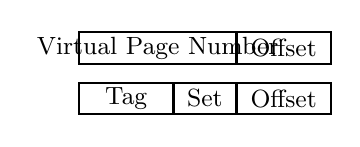
\begin{tikzpicture}[scale=0.8]
    \draw[thick] (0,0) rectangle (4,0.5);
    \draw[thick] (2.5,0) -- (2.5,0.5);
    \node at (1.25,0.25) {\small Virtual Page Number};
    \node at (3.25,0.25) {\small Offset};
    
    \draw[thick] (0,-0.8) rectangle (4,-0.3);
    \draw[thick] (1.5,-0.8) -- (1.5,-0.3);
    \draw[thick] (2.5,-0.8) -- (2.5,-0.3);
    \node at (0.75,-0.55) {\small Tag};
    \node at (2,-0.55) {\small Set};
    \node at (3.25,-0.55) {\small Offset};
\end{tikzpicture}

\textbf{On TLB miss:}\\
Page Miss Handler (PMH) gets PTE from memory
\end{column}

\begin{column}{0.4\textwidth}
\begin{center}
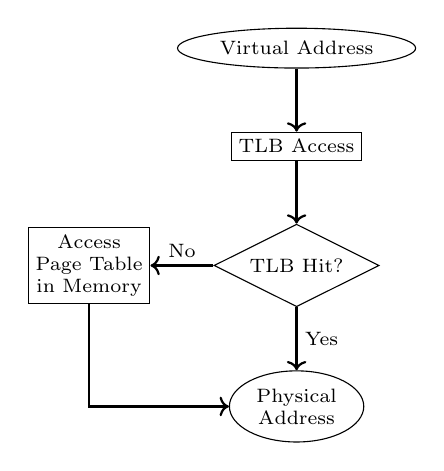
\begin{tikzpicture}[node distance=0.8cm, auto]
    \scriptsize
    % Nodes
    \node[draw, ellipse] (va) {Virtual Address};
    \node[draw, rectangle, below=of va] (tlb) {TLB Access};
    \node[draw, diamond, below=of tlb, aspect=2] (hit) {TLB Hit?};
    \node[draw, rectangle, left=of hit, align=center] (pt) {Access\\Page Table\\in Memory};
    \node[draw, ellipse, below=of hit, align=center] (pa) {Physical\\Address};
    
    % Arrows
    \draw[->, thick] (va) -- (tlb);
    \draw[->, thick] (tlb) -- (hit);
    \draw[->, thick] (hit) -- node[right] {Yes} (pa);
    \draw[->, thick] (hit) -- node[above] {No} (pt);
    \draw[->, thick] (pt) |- (pa);
\end{tikzpicture}
\end{center}
\end{column}
\end{columns}
\end{frame}

% Slide 10: STLB - Secondary TLB
\begin{frame}{STLB - Secondary TLB}
\begin{itemize}
    \item PMH can access STLB instead of performing page walk
    \item After TLB miss, look in STLB. The STLB is much larger than TLB, so it has higher hit rate but also higher access latency
    \item If hit on STLB, copy PTE to TLB
    \item STLB contains memory references from both I-cache and D-cache, allowing data and code pages to be shared
    \item Like TLB, uses VPN for lookup to STLB
    \item On STLB hit, translation is used
    \item On STLB miss, PMH performs page walk
\end{itemize}

\vspace{1em}
\textbf{TLB Hierarchy:}
\begin{center}
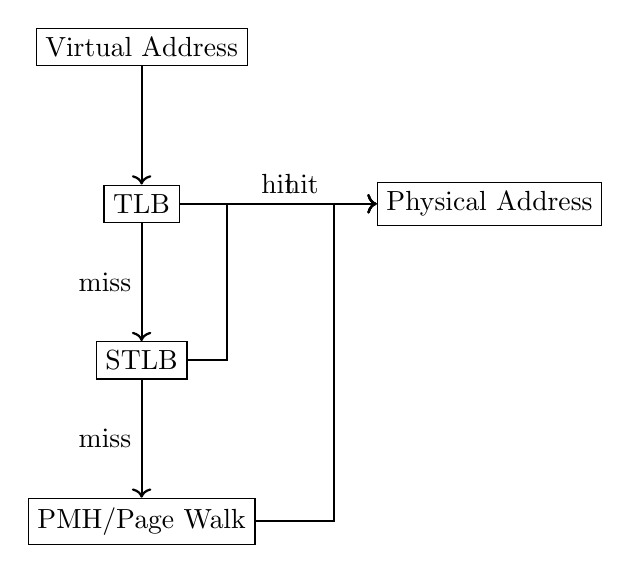
\begin{tikzpicture}[node distance=1.5cm, auto]
    \node[draw, rectangle] (va) {Virtual Address};
    \node[draw, rectangle, below=of va] (tlb) {TLB};
    \node[draw, rectangle, below=of tlb] (stlb) {STLB};
    \node[draw, rectangle, below=of stlb] (pmh) {PMH/Page Walk};
    \node[draw, rectangle, right=of tlb, xshift=1cm] (pa) {Physical Address};
    
    \draw[->, thick] (va) -- (tlb);
    \draw[->, thick] (tlb) -- node[left] {miss} (stlb);
    \draw[->, thick] (stlb) -- node[left] {miss} (pmh);
    \draw[->, thick] (tlb) -- node[above] {hit} (pa);
    \draw[->, thick] (stlb.east) -- ++(0.5,0) |- node[near end, above] {hit} (pa);
    \draw[->, thick] (pmh.east) -- ++(1,0) |- (pa);
\end{tikzpicture}
\end{center}
\end{frame}

% Slide 11: Virtual Memory and Cache
\begin{frame}{Virtual Memory and Cache}
\begin{center}
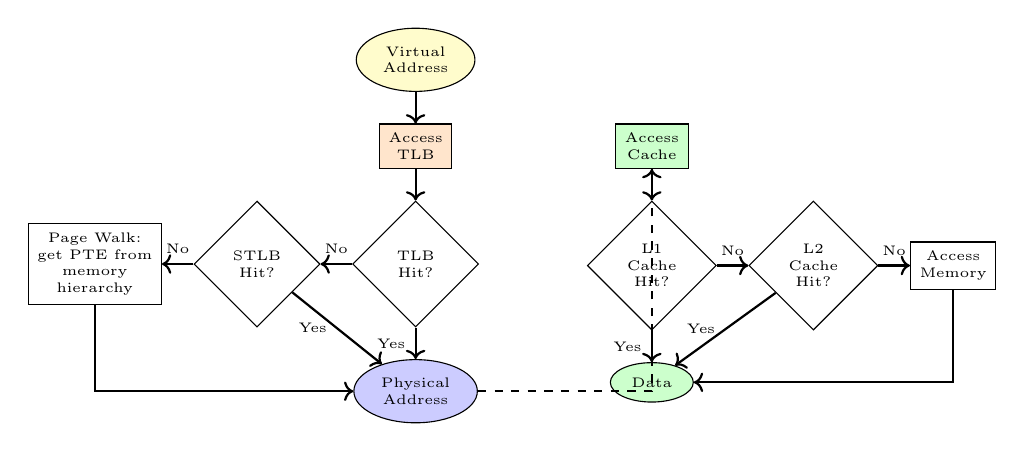
\begin{tikzpicture}[
    node distance=0.4cm and 0.4cm, 
    auto, 
    font=\tiny,
    diamond node/.style={draw, diamond, align=center, minimum width=1.6cm, minimum height=1.6cm}
]
    % Nodes
    \node[draw, ellipse, fill=yellow!20, align=center] (va) {Virtual\\Address};
    
    % TLB path
    \node[draw, rectangle, fill=orange!20, below=of va, align=center] (tlb) {Access\\TLB};
    \node[diamond node, below=of tlb] (tlbhit) {TLB\\Hit?};
    \node[diamond node, left=of tlbhit] (stlbhit) {STLB\\Hit?};
    \node[draw, rectangle, align=center, left=of stlbhit] (pw) {Page Walk:\\get PTE from\\memory\\hierarchy};
    
    % Cache path
    \node[draw, rectangle, fill=green!20, below=of va, xshift=3cm, align=center] (cache) {Access\\Cache};
    \node[diamond node, below=of cache] (l1hit) {L1\\Cache\\Hit?};
    \node[diamond node, right=of l1hit] (l2hit) {L2\\Cache\\Hit?};
    \node[draw, rectangle, right=of l2hit, align=center] (mem) {Access\\Memory};
    
    % Result nodes
    \node[draw, ellipse, fill=blue!20, below=of tlbhit, align=center] (pa) {Physical\\Address};
    \node[draw, ellipse, fill=green!20, below=of l1hit] (data) {Data};
    
    % Arrows - TLB path
    \draw[->, thick] (va) -- (tlb);
    \draw[->, thick] (tlb) -- (tlbhit);
    \draw[->, thick] (tlbhit) -- node[left] {Yes} (pa);
    \draw[->, thick] (tlbhit) -- node[above] {No} (stlbhit);
    \draw[->, thick] (stlbhit) -- node[above] {No} (pw);
    \draw[->, thick] (stlbhit) -- node[left] {Yes} (pa);
    \draw[->, thick] (pw) |- (pa);
    
    % Arrows - Cache path
    \draw[->, thick, dashed] (pa) -| (cache);
    \draw[->, thick] (cache) -- (l1hit);
    \draw[->, thick] (l1hit) -- node[left] {Yes} (data);
    \draw[->, thick] (l1hit) -- node[above] {No} (l2hit);
    \draw[->, thick] (l2hit) -- node[left] {Yes} (data);
    \draw[->, thick] (l2hit) -- node[above] {No} (mem);
    \draw[->, thick] (mem) |- (data);
\end{tikzpicture}
\end{center}

%\vspace{0.5em}
\begin{itemize}
    \item TLB access is serial with cache access
    \item Page table entries are cached in L1 D\$, L2\$, and L3\$ as data
\end{itemize}
\end{frame}

% Slide 12: Page Walk and PMH
\begin{frame}{Page Walk Process}
\textbf{PMH (Page Miss Handler) Operation:}
\begin{itemize}
    \item PMH performs page walk on TLB miss
    \item Walks the page table hierarchy from root (PML4)
    \item PMH contains caches for higher translation levels:
    \begin{itemize}
        \item PML4 cache
        \item PDP cache
        \item DIR cache
    \end{itemize}
\end{itemize}

\vspace{1em}
\textbf{PMH Cache Access:}
\begin{center}
\begin{tabular}{|l|c|c|}
\hline
\textbf{Cache} & \textbf{Accessed with} & \textbf{Returns} \\
\hline
DIR cache & [47:21] & PDE \\
PDP cache & [47:30] & PDP entry \\
PML4 cache & [47:39] & PML4 entry \\
\hline
\end{tabular}
\end{center}

\vspace{0.5em}
Note: No Table cache needed as TLB stores complete translations
\end{frame}

\begin{frame}{Caches and Translation Structures}
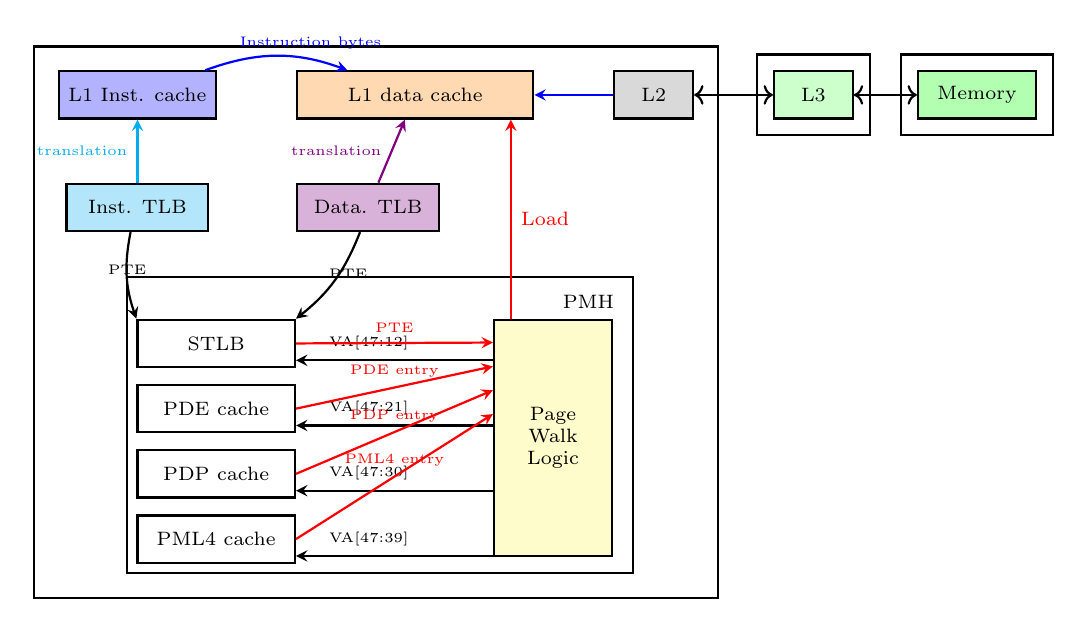
\begin{tikzpicture}[
    cache/.style={rectangle, draw, thick, minimum height=0.6cm, minimum width=2cm},
    tlb/.style={rectangle, draw, thick, minimum height=0.6cm, minimum width=1.8cm},
    bigbox/.style={rectangle, draw, thick},
    arrow/.style={->, >=stealth, thick,},
    label/.style={font=\tiny},
    font=\scriptsize
]

% L1 Caches
\node[cache, fill=blue!30] (l1inst) {L1 Inst. cache};
\node[cache, fill=orange!30, right=1cm of l1inst, minimum width=3cm] (l1data) {L1 data cache};

% TLBs
\node[tlb, fill=cyan!30, below=0.8cm of l1inst] (insttlb) {Inst. TLB};
\node[tlb, fill=violet!30, below=0.8cm of l1data.south west, anchor=north west] (datatlb) {Data. TLB};

% Translation caches
\node[cache, below=1.1cm of insttlb, xshift=1cm] (stlb) {STLB};
\node[cache, below=0.2cm of stlb] (pdecache) {PDE cache};
\node[cache, below=0.2cm of pdecache] (pdpcache) {PDP cache};
\node[cache, below=0.2cm of pdpcache] (pml4cache) {PML4 cache};

% PMH and Page Walk Logic
\node[rectangle, draw, thick, fill=yellow!20, minimum height=3cm, minimum width=1.5cm, 
      right=2.5cm of stlb, yshift=-1.2cm] (pmh) {};
\node[align=center, anchor=south west] (pmhlabel) at (pmh.north) {PMH};
\node[align=center] (pwllabel) at (pmh.center) {Page\\Walk\\Logic};

% Fit box around translation caches
\node[bigbox, fit=(stlb)(pdecache)(pdpcache)(pml4cache)(pmh)(pmhlabel)] (transbox) {};

% L2, L3, and Memory
\node[cache, fill=gray!30, right=of l1data, minimum width=1cm] (l2) {L2};
\node[cache, fill=green!20, right=of l2, minimum width=1cm] (l3) {L3};
\node[cache, fill=green!30, right=0.8cm of l3, minimum width=1.5cm] (memory) {Memory};

% Core box
\node[bigbox, fit=(l1inst)(l1data)(insttlb)(datatlb)(transbox)(pmhlabel)(l2), 
      inner sep=0.3cm, label={[font=\textbf]north west:Core}] (corebox) {};

% On-die box
\node[bigbox, fit=(l3), inner sep=0.2cm, label={[font=\small]above:On-die}] (ondiebox) {};

% Platform box
\node[bigbox, fit=(memory), inner sep=0.2cm, label={[font=\small]above:Platform}] (platformbox) {};

% Arrows and connections
\draw[arrow, blue] (l1inst) to[bend left=20] node[above, near end, label] {Instruction bytes} (l1data);
\draw[arrow, cyan] (insttlb) -- (l1inst) node[midway, left, label] {translation};
\draw[arrow, violet] (datatlb) -- (l1data) node[midway, left, label] {translation};

% PTE connections
\draw[arrow] (insttlb) to[bend right=15] node[near start, below, label] {PTE} (stlb.north west);
\draw[arrow] (datatlb) to[bend left=15] node[near start, below, label] {PTE} (stlb.north east);

\draw[arrow] ($(pmh.west |- stlb.south) + (0,1mm)$) -- node[near end, above, label, xshift=3mm] {VA[47:12]}  ($(stlb.south east) + (0,1mm)$);
\draw[arrow] ($(pmh.west |- pdecache.south) + (0,1mm)$) -- node[near end, above, label, xshift=3mm] {VA[47:21]}  ($(pdecache.south east) + (0,1mm)$);
\draw[arrow] ($(pmh.west |- pdpcache.south) + (0,1mm)$) -- node[near end, above, label, xshift=3mm] {VA[47:30]}  ($(pdpcache.south east) + (0,1mm)$);
\draw[arrow] ($(pmh.west |- pml4cache.south) + (0,1mm)$) -- node[near end, above, label, xshift=3mm] {VA[47:39]}  ($(pml4cache.south east) + (0,1mm)$);

% From translation caches to PMH
\draw[arrow, red, thick] (stlb.east) -- node[above, label] {PTE} 
      ($(pmh.west)!0.8!(pmh.north west)$);
\draw[arrow, red, thick] (pdecache.east) -- node[above, label] {PDE entry} 
      ($(pmh.west)!0.6!(pmh.north west)$);
\draw[arrow, red, thick] (pdpcache.east) -- node[above, label] {PDP entry} 
      ($(pmh.west)!0.4!(pmh.north west)$);
\draw[arrow, red, thick] (pml4cache.east) -- node[above, label] {PML4 entry} 
      ($(pmh.west)!0.2!(pmh.north west)$);

% VA labels on the right side of PMH
%\node[label, right=0.1cm of pmh.east, yshift=1.2cm] {VA[47:12]};
%\node[label, right=0.1cm of pmh.east, yshift=0.4cm] {VA[47:21]};
%\node[label, right=0.1cm of pmh.east, yshift=-0.4cm] {VA[47:30]};
%\node[label, right=0.1cm of pmh.east, yshift=-1.2cm] {VA[47:39]};

% PMH to L1 data cache
%\draw[arrow, red, thick] (pmh.north) to[out=90, in=270] (l1data.south);
\draw[arrow, red, thick] 
  ($(pmh.north -| l1data.east) + (-3mm,0)$) --  
  node[right, align=center] {Load} 
  ($(l1data.south east) + (-3mm,0)$);


% L1 data cache to L2
\draw[arrow, blue, thick] (l2.west) -- (l1data.east);

% L2 to L3 to Memory
\draw[<->, thick] (l2.east) -- (l3.west);
\draw[<->, thick] (l3.east) -- (memory.west);

\end{tikzpicture}
\end{frame}


% Slide 13: Question 2 Setup
\begin{frame}{Question 2}
\textbf{System Configuration:}
\begin{itemize}
    \item Processor similar to X86-64
    \item 4KB pages
    \item TLB present (Hit: immediate translation, Miss: Page Walk required)
    \item PMH contains cache for each translation table level
    \item All caches and TLB empty on reset
\end{itemize}

\vspace{1em}
\textbf{Memory Access Sequence:}
\begin{center}
\begin{tabular}{|l|c|l|}
\hline
\textbf{Address} & \textbf{Memory Accesses} & \textbf{Explanation} \\
\hline
0x0000022334455666 & ? & \\
0x0000022334455777 & ? & \\
0x0000022884455777 & ? & \\
\hline
\end{tabular}
\end{center}
\end{frame}

% Slide 14: Question 2 Solution
\begin{frame}{Question 2 - Solution}
\begin{center}
\begin{tabular}{|l|c|p{6cm}|}
\hline
\textbf{Address} & \textbf{Accesses} & \textbf{Explanation} \\
\hline
0x0000022334455666 & 4 & Need to access memory for each of the 4 translation tables \\
\hline
0x0000022334455777 & 0 & Same page as above $\Rightarrow$ TLB hit $\Rightarrow$ No memory access \\
\hline
0x0000022884455777 & 3 & Hit in PML4 cache, then miss in PDP. Need to access memory 3 times: PDP, DIR, PTE \\
\hline
\end{tabular}
\end{center}
\end{frame}

% Slide 15: Cache Design Question
\begin{frame}{Question 2: Cache Design}
\textbf{System Configuration:}
\begin{itemize}
    \item Virtual address: 48 bits
    \item Physical address: 41 bits
    \item L1 data cache: 32KB, 2-way set associative, 64B line size
\end{itemize}

\vspace{1em}
\textbf{Question:} How can we access this cache before getting the physical address?

\vspace{1em}
\textbf{Analysis:}
\begin{itemize}
    \item 64B lines $\Rightarrow$ 6 offset bits [5:0]
    \item $\frac{32\text{KB}}{(2\text{ ways} \times 64\text{B})}$ = 256 sets $\Rightarrow$ 8 set bits [13:6]
    \item 12 bits [11:0] are not translated (page offset)
    \item We lack 2 bits [13:12] for complete set address
    \item Solution: Use untranslated bits [13:12] for set lookup
    \item Must compare entire PFN with tag due to aliasing possibility
\end{itemize}
\end{frame}

% Slide 16: Virtual Aliasing Problem
\begin{frame}{Virtual Aliasing Problem}
\textbf{Problem:} Two virtual pages mapping to same physical page

\vspace{1em}
Example:
\begin{itemize}
    \item VPN xxxx01 $\rightarrow$ PFN zzzz
    \item VPN yyyy00 $\rightarrow$ PFN zzzz
    \item Bits [13:12] differ (01 vs 00)
\end{itemize}

\vspace{1em}
\textbf{Consequence:}
\begin{itemize}
    \item Same data may exist in two different cache sets
    \item Violates cache coherency
\end{itemize}

\vspace{1em}
\textbf{Solution:}
\begin{itemize}
    \item Check 4 possible sets when allocating new entry
    \item If same tag appears, evict the alias
    \item On snoop: must check 4 sets × 2 ways = 8 locations
\end{itemize}
\end{frame}

% Slide 17: Question 3 Setup
\begin{frame}{Question 3}
\textbf{System Configuration:}
\begin{itemize}
    \item Core similar to X86 in 64-bit mode
    \item Entry size in all page tables: 8 bytes
    \item PMH caches at all levels:
    \begin{itemize}
        \item 4 entries, direct mapped
        \item Hit time: 2 cycles
        \item Miss detected after 1 cycle
    \end{itemize}
    \item Main memory access: 100 cycles (not including miss detection)
    \item All PMH levels accessed in parallel
\end{itemize}

\vspace{0.1em}
\textbf{Address format:} \vmaddressbreakdown{8}{20}{12}{12}{0}{12}

\vspace{0.1em}
\textbf{Questions:}
\begin{enumerate}
    \item What is the large page size?
    \item How many entries in each table?
\end{enumerate}
\end{frame}

% Slide 18: Question 3 Solution Part 1
\begin{frame}{Question 3 - Solution Part 1}
\textbf{1. Large page size:}
\begin{itemize}
    \item Large pages pointed by DIR
    \item Offset bits: [23:0]
    \item Size = $2^{24}$ = 16MB
\end{itemize}

\vspace{1em}
\textbf{2. Entries per table:}
\begin{itemize}
    \item TABLE: $2^{12}$ bits offset $\Rightarrow 2^{12}$ entries
    \item DIR: $2^{12}$ bits $\Rightarrow 2^{12}$ entries  
    \item PDP: $2^{12}$ bits $\Rightarrow 2^{12}$ entries
    \item PML4: $2^{8}$ bits $\Rightarrow 2^{8}$ = 256 entries
\end{itemize}
\end{frame}

% Slide 19: Question 3 Memory Access Analysis
\begin{frame}{Question 3 - Memory Access Analysis}
\footnotesize
% Define colors for different page table levels
\definecolor{signcolor}{RGB}{128,128,128}
\definecolor{pml4color}{RGB}{255,128,0}
\definecolor{pdpcolor}{RGB}{51,153,255}
\definecolor{dircolor}{RGB}{0,204,102}
\definecolor{offsetcolor}{RGB}{204,0,204}

\begin{center}
\begin{tabular}{|l|c|p{8cm}|}
\hline
\textbf{Virtual Address} & \textbf{Cycles} & \textbf{Comment} \\
\hline
\textcolor{signcolor}{0xFF81}\textcolor{pml4color}{234}\textcolor{pdpcolor}{567}\textcolor{dircolor}{89A}\textcolor{offsetcolor}{BCD} & \onslide<2->{401} & \onslide<2->{Miss at each level: 1 + 4 $\times$ 100 = 401 cycles} \\
\hline
\textcolor{signcolor}{0xFF81}\textcolor{pml4color}{234}\textcolor{pdpcolor}{067}\textcolor{dircolor}{89A}\textcolor{offsetcolor}{BCD} & \onslide<3->{202} & \onslide<3->{(PML4, PDP, DIR, TLB) = (H,H,M,M)}\\
& & \onslide<3->{1 cycle + PDP read 1 cycle}\\
& & \onslide<3->{DIR miss: 100 cycles, PTE miss: 100 cycles} \\
\hline
\textcolor{signcolor}{0xFF80}\textcolor{pml4color}{234}\textcolor{pdpcolor}{067}\textcolor{dircolor}{89A}\textcolor{offsetcolor}{BCD} & \onslide<4->{401} & \onslide<4->{PMH cache miss in all levels: 1 + 4 $\times$ 100 = 401} \\
\hline
\textcolor{signcolor}{0xFF81}\textcolor{pml4color}{234}\textcolor{pdpcolor}{067}\textcolor{dircolor}{09A}\textcolor{offsetcolor}{BCD} & \onslide<5->{302} & \onslide<5->{(PML4, PDP, DIR, TLB) = (H,M,M,M)}\\
& & \onslide<5->{Entry 234 replaced by access 3 (same set)}\\
& & \onslide<5->{2 + 3 $\times$ 100 = 302 cycles} \\
\hline
\textcolor{signcolor}{0xFF81}\textcolor{pml4color}{234}\textcolor{pdpcolor}{067}\textcolor{dircolor}{09A}\textcolor{offsetcolor}{0CD} & \onslide<6->{2} & \onslide<6->{Hit in TLB - 2 cycles} \\
\hline
\end{tabular}
\end{center}

\vspace{0.5em}
\onslide<7->{
\small
\textbf{Color Legend:} 
\textcolor{signcolor}{Sign}, 
\textcolor{pml4color}{PML4}, 
\textcolor{pdpcolor}{PDP}, 
\textcolor{dircolor}{DIR}, 
\textcolor{offsetcolor}{Offset}
}
\end{frame}

% Final slide: Summary
\begin{frame}{Summary}
\begin{itemize}
    \item \textbf{x86 Virtual Memory Hierarchy}
    \begin{itemize}
        \item Multi-level page tables: PML4 $\rightarrow$ PDP $\rightarrow$ DIR $\rightarrow$ TABLE
        \item Efficient memory usage through dynamic allocation
        \item Support for multiple page sizes: 4KB, 2MB, 1GB
    \end{itemize}

    \vspace{0.5em}
    \item \textbf{TLB (Translation Lookaside Buffer)}
    \begin{itemize}
        \item Hardware cache for page table entries
        \item Critical for performance: avoids multiple memory accesses
        \item Must consider hit/miss patterns in access analysis
    \end{itemize}

    \vspace{0.5em}
    \item \textbf{Key Design Considerations}
    \begin{itemize}
        \item Entry size determines entries per table
        \item Address field widths depend on table size
        \item PMH (Page Miss Handler) caching impacts latency
        \item Sign extension for 64-bit addressing
    \end{itemize}
\end{itemize}
\end{frame}

\end{document}